%! Author = michael
%! Date = 08.10.20

% Preamble
\documentclass[11pt]{article}
\usepackage{pdfpages}
\usepackage[german]{babel}
\usepackage{amsmath}
\usepackage[backend=biber]{biblatex}
\usepackage{csquotes}
\usepackage{changepage}
\usepackage{graphicx}
\usepackage{listings}
\usepackage{xcolor}

\definecolor{codegreen}{rgb}{0,0.6,0}
\definecolor{codegray}{rgb}{0.5,0.5,0.5}
\definecolor{codepurple}{rgb}{0.58,0,0.82}
\definecolor{backcolour}{rgb}{0.95,0.95,0.92}

\lstdefinestyle{code}{
backgroundcolor=\color{backcolour},
commentstyle=\color{codegreen},
keywordstyle=\color{magenta},
numberstyle=\tiny\color{codegray},
stringstyle=\color{codepurple},
basicstyle=\ttfamily\footnotesize,
breakatwhitespace=false,
breaklines=true,
captionpos=b,
keepspaces=true,
numbers=left,
numbersep=5pt,
showspaces=false,
showstringspaces=false,
showtabs=false,
tabsize=2
}

\lstset{style=code}


\setlength{\parindent}{0em}
\setlength{\parskip}{0.8em}

\addbibresource{main.bib}

% Document
\begin{document}
    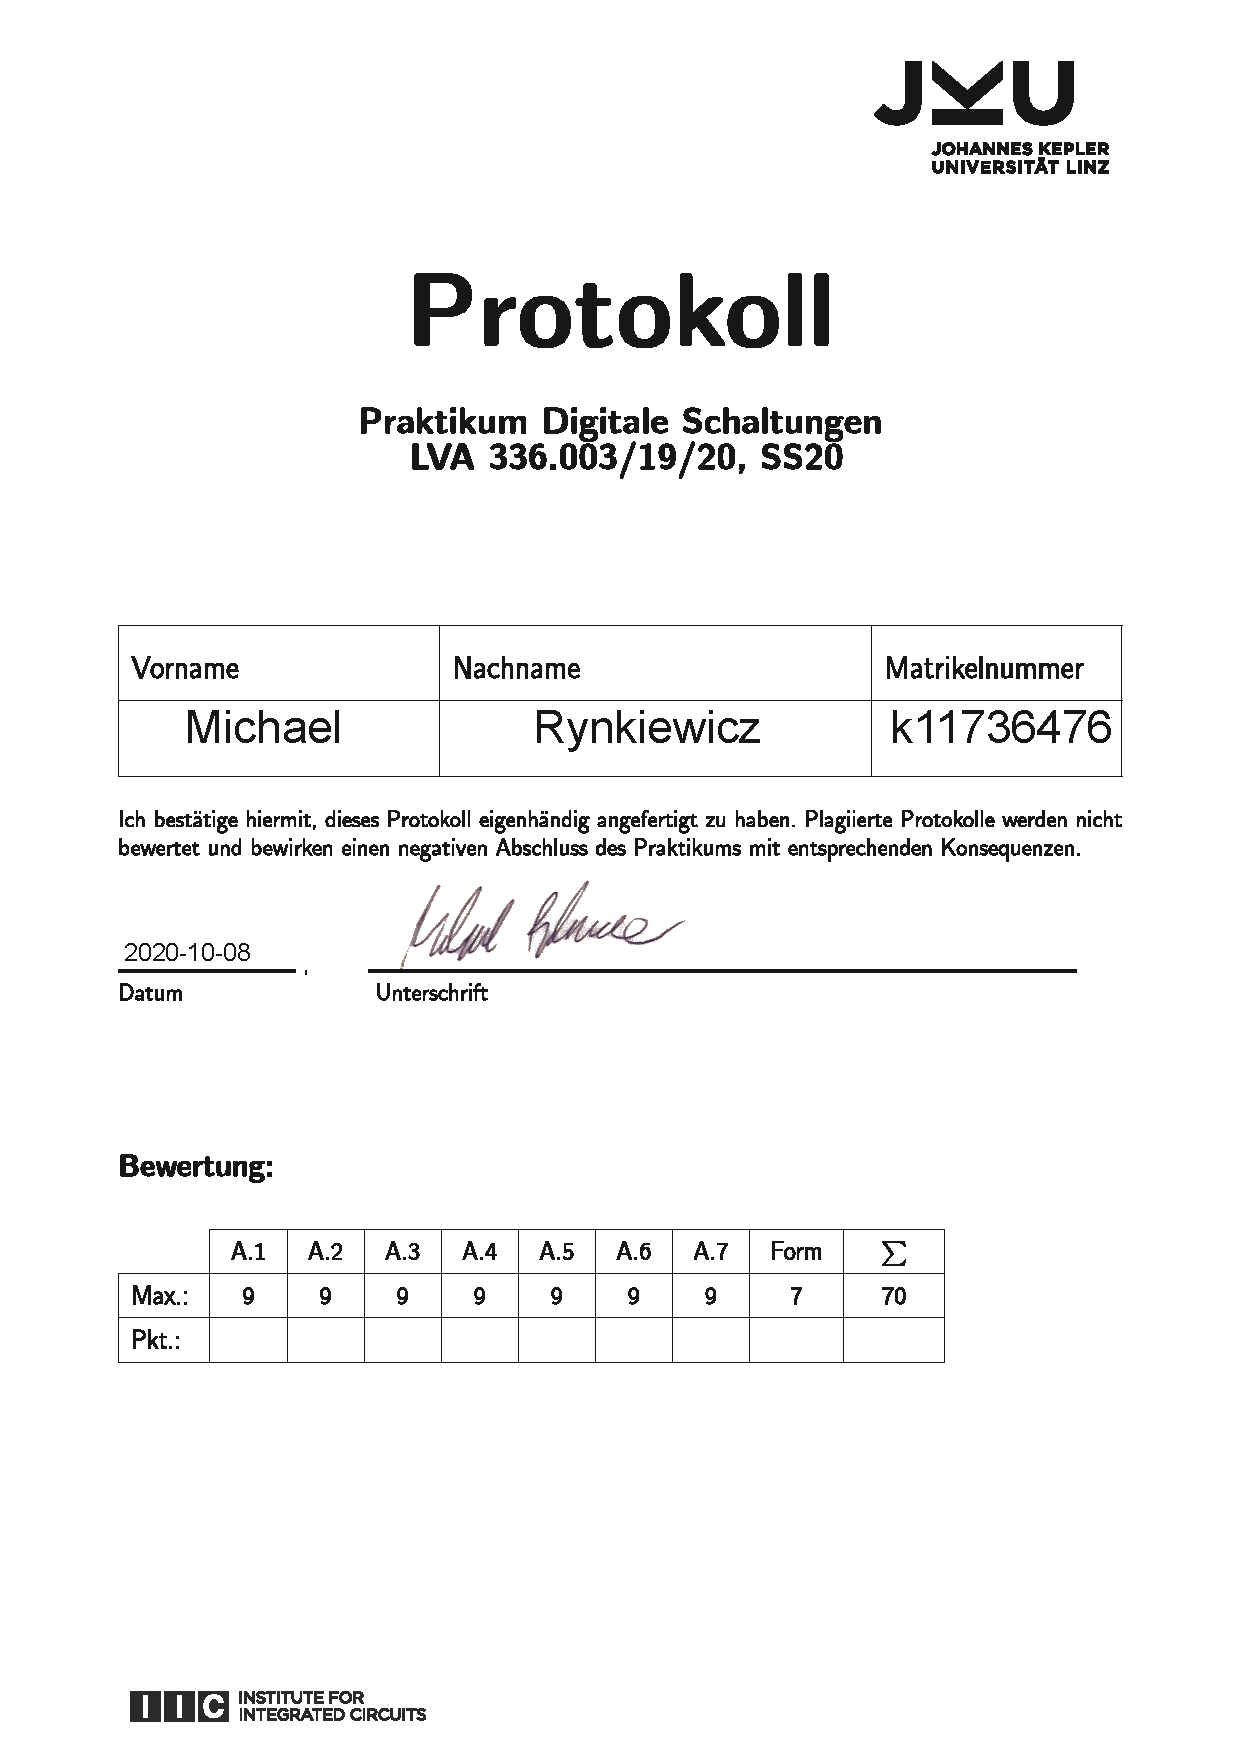
\includepdf[pages=-]{deckblatt.pdf}

    \tableofcontents
    \newpage

    

\section{Einleitung}
\label{sec:einleitung}

Das Wissen um die Funktionsweise eines Mikrocontrollers ist wesentlicher Bestandteil eines Informatik-Studiums.
Im Zuge Dieses werden in diesem Protokoll verschiedene Experimente beschrieben und evaluiert.
Insgesamt werden sieben Experimente begutachtet und diskutiert, welche im Zeitraum vom 28.September 2020 und 2.Oktober 2020 durchgeführt wurden.


\section{Verwendete Materialien}
\label{sec:verwendete-materialien}

Jede Sektion gibt die in ihr verwendeten Materialien mitsamt ihrer Stückzahl an.
In dieser Sektion werden alle Materialien im Allgemeinen gelistet und beschrieben.

\subsection{LED}
\label{subsec:led}
Eine Leuchtdiode (LED) ist ein Bauelement der Elektronik.
Wird sie von elektrischen Strom durchflossen beginnt sie Licht auszustrahlen.
Die Wellenlänge, d.h., die Farbe des Lichts sowie ob es für das menschliche Auge sichtbar ist oder nicht, hängt von den benutzten Materialien im inneren der LED ab.
Die in der LED verwendeten Materialien sind für dieses Protokoll nicht weiter von Bedeutung.
Für die beschriebenen Aufgaben wurden die folgenden LEDs verwendet.

\begin{table}[h]
    \centering
    \caption{LEDs - Farben, Flussspannung, Maximalstrom \cite{led-elektrische-eigenschaften}}
    \label{tab:leds-farben-und-elemente}
    \begin{tabular}{| l | l | l |}
        \hline
        Farbe & Durchflussspannung & Maximalstrom \\
        \hline
        Rot   & 1,6V - 2,2V        & 20mA         \\
        Gelb  & 1,9V - 2,5V        & 20mA         \\
        Grün  & 1,9V - 2,5V        & 20mA         \\
        \hline
    \end{tabular}
\end{table}

\subsection{Widerstände}
\label{subsec:widerstände}

Widerstände werden verwendet, um einen Spannungsabfall in einem Stromkreis zu verursachen.
Damit kann die Stromstärke in einem Stromkreis begrenzt beziehungsweise verringert werden.
Oft wird bei der Verwendung von LEDs ein sogenannter Vorwiederstand verwendet, um die Stromstärke soweit abzusenken, dass die LED nicht beschädigt wird.

In den Aufgaben wurden Widerstände der sogenannten E6-Reihe verwendet.
E-Reihen sind normierte Widerstandsgrößen, wobei die Zahl die Stufen zwischen den Potenzen angibt.
D.h., bei der E6-Reihe sind sechs verschiedene Widerstandsgrößen zwischen $10\Omega$ und $100\Omega$, zwischen $100\Omega$ und $1000\Omega$, u.s.w. bis zum oberen Limit von $10M\Omega$.

Die verwendeten Widerstände sind Farbcodiert, um sie voneinander unterscheiden zu können.
Die Farbkodierung von Widerständen wird in den Aufgaben, in denen sie verwendet werden, angegeben.
Die Bedeutung der Codierung der verwendeten Widerstände kann in Tab. \ref{tab:farbcodierung-von-widerständen} abgelesen werden.

\begin{table}
    \begin{adjustwidth}{-2cm}{}
        \caption{Farbcodierung von Widerständen}
        \label{tab:farbcodierung-von-widerständen}
        \begin{tabular}{| l | l | l | l | l |}
            \hline
            Farbe & 1.Ring (10er Stelle) & 2.Ring (1er Stelle) & 3.Ring (Multiplikator) & 4.Ring (Toleranz) \\
            \hline
            Braun & 1                    & 0                   & 10                     & $\pm 1$           \\
            Grün  & 5                    & 5                   & $100\ 000$             & $\pm 0.5$         \\
            Gold  & -                    & -                   & $0.1$                  & $\pm 5$           \\
            \hline
        \end{tabular}
    \end{adjustwidth}
\end{table}

\subsection{Taster}
\label{subsec:taster}

\subsection{Mikrocontroller \cite{arduino-r3}}
\label{subsec:mikrocontroller}

Mikrocontroller werden verwendet, um komplexere Logik in eine elektronische Schaltung zu integrieren.
Die in diesem Protokoll verwendete Mikrocontroller sind Mikrocontroller vom Typ Arduino Uno Rev 3.
Diese Mikrocontroller besitzen 14 digitale Pins, an denen eine Spannung von entweder 0V oder 5V angelegt oder ausgegeben werden kann.
Des Weiteren besitzt es sechs analoge Pins, welche auch auf Spannungsschwankungen reagieren können.
Weitere wichtige Pins sind In-Pins, welche eine Spannung von 5V liefern können und Out-Pins, welche eine Verbindung zur Erdung herstellen.

\subsection{Logikbausteine}
\label{subsec:logikbausteine}

Um verschiedene Logikgatter in Schaltungen verwenden zu können, ohne komplizierte Schaltkreise bauen zu müssen, werden Logikbausteine verwenden.
Diese Bausteine implementieren verschiedene Gatter.
D.h., bei zwei Eingängen $a$ und $b$, wird durch das Anwenden der Funktion, die der Baustein implementiert,  der Ausgang $y$ erzeugt.
Diese Funktionen bilden logische Operationen ab.
Die Erklärung von logischen Funktionen würden über den Umfang dieses Protokolls hinausgehen und werden daher nicht weiter erklärt.
In Tabelle \ref{tab:bausteine-und-deren-logische-funktionen} sind die verwendeten Bausteine und die Funktionen die sie implementieren gelistet.

\begin{table}[ht]
    \centering
    \caption{Bausteine und deren logische Funktionen}
    \label{tab:bausteine-und-deren-logische-funktionen}
    \begin{tabular}{| l | l |}
        \hline
        Bausteinbezeichnung & Funktion \\
        \hline
        74HC00 & NAND \\
        74HC02 & NOR \\
        74HC08 & AND \\
        74HC32 & OR \\
        74HC86 & XOR \\
        \hline
    \end{tabular}
\end{table}

\section{Begriffe}
\label{sec:begriffe}

\subsection{Pulsewellenmodulation (PWM)}
\label{subsec:pulsewellenmodulation-(pwm)}

\subsection{PullUp}
\label{subsec:pullup}

\subsection{Baudrate}
\label{subsec:baudrate}

\subsection{Wahrheitstabelle}
\label{subsec:wahrheitstabelle}


    \section{Aufgabe 1 - Ampelsteuerung}
\label{sec:aufgabe-1}

Es soll eine Ampelsteuerung implementiert und getestet werden.
Die Ampel wird mithilfe von drei LEDs, in den Farben Rot, Gelb und Grün, aufgebaut.
Weiters soll die Steuerung folgende Funktionsweise implementieren:

\textbf{Phase 1} soll die Ampel auf Rot setzen.
D.h., die rote LED wird eingeschaltet.
Dieser Zustand soll vier Sekunden lang gehalten werden.

\textbf{Phase 2} soll zusätzlich zur roten LED die gelbe einschalten.
Dieser Zustand soll eine Sekunde lang gehalten werden.

\textbf{Phase 3} soll die rote sowie die gelbe LED ausschalten, während die Grüne eingeschaltet wird.
Dieser Zustand soll vier Selunden lang gehalten werden.

\textbf{Phase 4} soll die grüne LED ausschalten während die Gelbe eingeschaltet wird.
Dieser Zustand soll eine Sekunde lang gehalten werden.
Nach Ablauf der vier Sekunden soll die grüne LED erlöschen und der Ablauf bei Phase 1 neu gestartet werden.

\subsection{Materialien}
\label{subsec:A1-materialien}

\begin{table}[h]
    \centering
    \caption{Aufgabe 1 - Verwendete Materialien}
    \label{tab:a1-materialien}
    \begin{tabular}{| l | l | l |}
        \hline
        Bezeichnung & Eigenschaften & Menge \\
        \hline
        Widerstand  & $150\Omega$   & 3     \\
        & Braun - Grün - Braun - Gold & \\
        LED & Rot & 1 \\
        LED & Gelb & 1 \\
        LED & Grün & 1 \\
        Mikrocontroller & Arduino Uno R3 & 1 \\
        \hline
    \end{tabular}
\end{table}

\newpage

\subsection{Vorbereitung}
\label{subsec:A1-vorbereitung}

Für den Schaltkreis müssen die Vorwiederstände für die LEDs berechnet werden.
Folgende Angaben sind bekannt.

\begin{itemize}
    \item Ausgangsspannung der Pins des Mikrocontrollers: $V_{out} = 5V$
    \item Diodenspannung der LEDs: $U_D = 2V$
    \item Diodenstrom der LEDs: $I_D = 15mA$
\end{itemize}

Zur Berechnung wird folgender Stromkreis angenommen.

\begin{figure}[h]
    \centering
    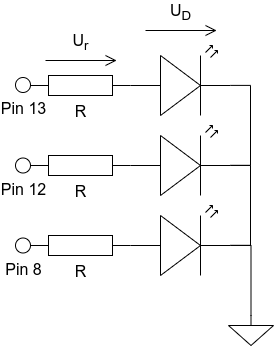
\includegraphics[height=0.4\textheight]{pictures/A1.png}
    \caption{Stromkreis A1}
    \label{fig:stromkreis-a1}
\end{figure}

Die Formel zur Berechnung des Stroms durch eine Diode ist bekannt.

\begin{equation}
    I_D =  \frac{1}{R_d} * (U - U_D) \label{eq:diodenstrom}
\end{equation}

Damit kann der benötigte Vorwiderstand berechnet werden.

\begin{equation}
    \begin{align}
        I_D =  \frac{1}{R_D} * (U - U_D) \Rightarrow \\
        R_D = \frac{1}{I_D} * (U - U_D) \\
        = \frac{1}{15mA} * (5V - 2V) \\
        = 200\Omega
    \end{align}
    \label{eq:equation-a1}
\end{equation}

Nachdem in der E6 Reihe keine $200\Omega$ Widerstände vorhanden sind, wurden $150\Omega$ gewählt.
Diese Wahl erfolgt aus folgenden Überlegungen.

\begin{enumerate}
    \item Laut angabe benötigt die LED $2V$ um zu schalten.
    \item Es existieren die Widerstände $150\Omega$ und $220\Omega$ in der E6-Reihe
    \item Bei einem Widerstand von $220\Omega$ würden, laut Gleichung \ref{eq:diodenstrom}, $I_D = \frac{3V}{220\Omega} = 13,636mA$ durch die LED fließen.
    \item Bei einem Widerstand von $150\Omega$ würden, laut Gleichung \ref{eq:diodenstrom}, $I_D = \frac{3V}{150\Omega} = 20mA$ durch die LED fließen.
\end{enumerate}
Da die Leuchtkraft einer LED von der Stromstärke abhängt und der Maximalstrom bei $20mA$ liegt, wurden $150\Omega$ gewählt.
Bei dieser Größe wird die LED bei theoretisch voller Leuchtkraft betrieben ohne die Lebensdauer markant zu verkürzen.

\subsection{Praktikumsaufgabe}
\label{subsec:praktikumsaufgabe}

Der Stromkreis wurde laut Abbildung \ref{fig:stromkreis-a1} implementiert.
Die Implementierung wird in Abbildung \ref{fig:implementierung-a1} gezeigt.

\begin{figure}[h]
    \centering
    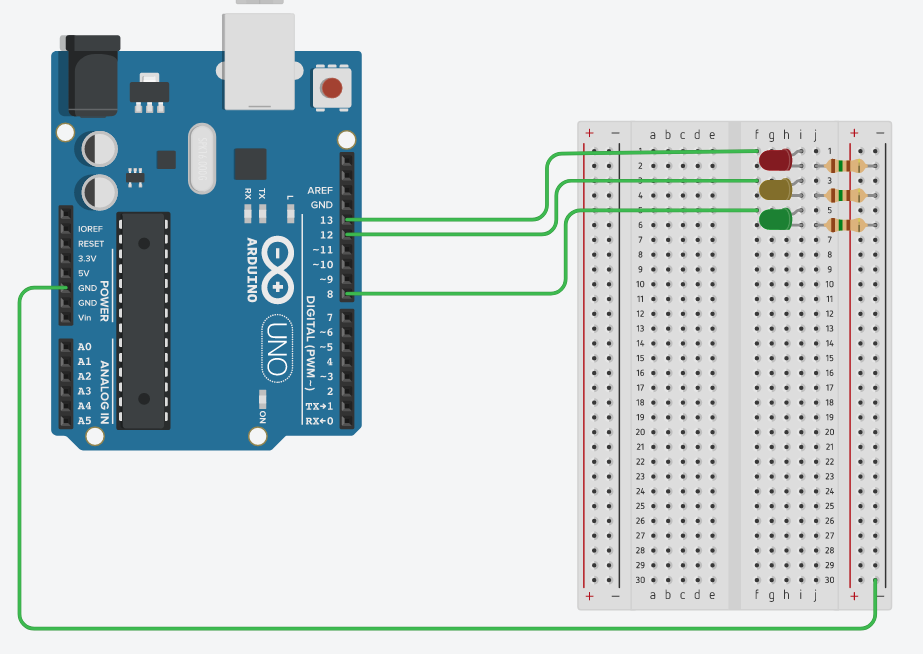
\includegraphics[width=\textwidth]{pictures/a1-praktik.png}
    \caption{Implementiert Stromkreis von Aufgabe 1}
    \label{fig:implementierung-a1}
\end{figure}

Wie in Abbildung \ref{fig:implementierung-a1} gezeigt, wurden die Pins 13, 12 und 8 gewählt.
Für die Wahl wurden die digitalen Pins herangezogen, da eine analoge Ausgabe nicht erforderlich war.
Die Pins die mit einer Tilde ($\sim$) markiert sind, sind in der Lage ein PWM-Signal zu liefern.
Da ein solches Signal nicht benötigt wird, wurden auch diese ausgeschlossen.
Von oben nach unten betrachte, wurden nun drei Pins ausgewählt, diese sind 13, 12, und 8.
Die genannten Pins werden, im Code, als digitale Output-Pins konfiguriert.

Im nachfolgendem Text wird der Programmcode der Aufgabe erläutert.
Einzelne Teile des Codes werden ausgewählt und beschrieben.
Am Ende dieser Sektion befindet sich der vollständige Programmcode.

\begin{lstlisting}[language=C,label={lst:a1-konstanten}, caption={Konstanten für Aufgabe 1}]
const int PIN_RED = 13;
const int PIN_YELLOW = 12;
const int PIN_GREEN = 8;
\end{lstlisting}

In Listing \ref{lst:a1-konstanten} werden die Pins definiert.
Durch das Anlegen von Konstanten für die Pins, kann der Code aussagekräftiger gestaltet werden.
Des weiteren entsteht dadurch die Möglichkeit, andere Pins zu verwenden, ohne den gesamtem Code durchgehen zu müssen.
Es reicht die Nummer an einer Stelle zu ändern.

\newpage

\begin{lstlisting}[language=C,label={lst:a1-setup}, caption={Setup für Aufgabe 1}]
void setup()
{
  pinMode(PIN_RED, OUTPUT);
  pinMode(PIN_YELLOW, OUTPUT);
  pinMode(PIN_GREEN, OUTPUT);
}
\end{lstlisting}

In Listing \ref{lst:a1-setup} werden die Pins angelegt und konfiguriert.
Wie oben beschrieben werden die Pins als Output-Pins, d.h., als Spannungsquelle, angelegt.

\begin{lstlisting}[language=C,label={lst:a1-onoff}, caption={On- und Off Methoden für Aufgabe 1}]
void off(int pin) {
  digitalWrite(pin, LOW);
}

void on(int pin) {
  digitalWrite(pin, HIGH);
}
\end{lstlisting}

In Listing \ref{lst:a1-onoff} werden die Pins entweder ausgeschalten (LOW) oder eingeschalten (HIGH).
Durch das Verwenden dieser Methoden ist es einfacher, die Phasen zu definieren bzw., im Code zu erkennen.

\begin{lstlisting}[language=C,label={lst:a1-loop}, caption={Programmschleife für Aufgabe 1}]
void loop()
{
  off(PIN_YELLOW);
  on(PIN_RED);
  delay(4 * 1000);

  on(PIN_YELLOW);
  delay(1 * 1000);

  off(PIN_RED);
  off(PIN_YELLOW);
  on(PIN_GREEN);
  delay(4 * 1000);

  off(PIN_GREEN);
  on(PIN_YELLOW);
  delay(1 * 1000);
}
\end{lstlisting}

\newpage

In Listing \ref{lst:a1-loop} werden die einzelnen Phasen implementiert.
Nach jeder Leerzeile, d.h., nach Zeile 6, 9, und 14 beginnt jeweils eine neue Phase.

Zu Beginn wird Phase 1 implementiert.
Diese Schaltet die gelbe LED, Pin 12, aus, falls vorher Phase 4 aktiv war und schaltet die rote LED, Pin 13, an.
Danach wird die $delay(x)$ Funktion aufgerufen, welche die Programmausführung für $x$ Millisekunden unterbricht.
Die Angabe von $x$ als Berechnung aus $Sekunde * 1000$ wurde gewählt, um im Code besser erkenntlich zu machen, dass es sich um Millisekunden handelt.
Der Programmfluss wird daher für vier Sekunden unterbrochen.

Dann folgt Phase 2, welche zusätzlich zur Roten auch die gelbe LED einschaltet.
Der Programmfluss wird für eine Sekunde unterbrochen.

Es folgt Phase 3.
Die Rote und die gelbe LED werden ausgeschaltet.
Die Grüne, Pin 8, wird eingeschaltet.
Der Programmfluss wird für weitere vier Sekunden unterbrochen.

Schlussendlich folgt Phase 4.
Es wird die grüne LED wieder ausgeschaltet, während die Gelbe aktiv wird.
Es folgt wieder eine Unterbrechung des Programms für eine Sekunde.
Am Ende der $loop()$ Funktion wird sie wieder von Beginn an, d.h., von Phase 1 aus, ausgeführt.

\newpage
\begin{lstlisting}[language=C,label={lst:a1-programmcode}, caption={Vollständiger Programmcode für Aufgabe 1}]
const int PIN_RED = 13;
const int PIN_YELLOW = 12;
const int PIN_GREEN = 8;

void setup()
{
  pinMode(PIN_RED, OUTPUT);
  pinMode(PIN_YELLOW, OUTPUT);
  pinMode(PIN_GREEN, OUTPUT);
}

void loop()
{
  off(PIN_YELLOW);
  on(PIN_RED);
  delay(4 * 1000);

  on(PIN_YELLOW);
  delay(1 * 1000);

  off(PIN_RED);
  off(PIN_YELLOW);
  on(PIN_GREEN);
  delay(4 * 1000);

  off(PIN_GREEN);
  on(PIN_YELLOW);
  delay(1 * 1000);
}

void off(int pin) {
  digitalWrite(pin, LOW);
}

void on(int pin) {
  digitalWrite(pin, HIGH);
}
\end{lstlisting}

\subsection{Fehlerdiskussion}
\label{subsec:a1-fehlerdiskussion}

Es wurden während dieser Aufgabe keine Fehler gefunden.


    
\section{Aufgabe 2 - Reaktionsspiel}
\label{sec:aufgabe-2---reaktionsspiel}

Es soll eine Schaltung implementiert werden, welche ein lichtbasiertes Reaktionsspiel darstellt.
Die Schaltung soll aus fünf LEDs bestehen, welche der Reihe nach leuchten und erlöschen.
D.h., LED 1 leuchtet, LED 1 erlischt und LED 2 leuchtet, LED 2 erlischt und LED 3 leuchtet, u.s.w..
Sobald die letzte LED erlischt soll die erste LED wieder leuchten und der Rythmus von neuen beginnen.

Die LEDs werden in der Reihenfolge Rot - Gelb - Grün - Gelb - Rot geschaltet und angeordnet.
Des weiteren wird ein Taster eingebaut.
Wird der Taster gedrückt, wenn die grüne LED leuchtet, halbiert sich die Zeit zwischen der die LEDs geschaltet werden.
D.h., bleibt eine LED fünf Sekunden eingeschaltet, bevor die nächste LED geschaltet wird, so bleibt sie danach nur 2,5 Sekunden lang eingeschaltet.
Wird der Taster erneut gedrückt, wenn die grüne LED leichtet, halbiert sich die Zeit erneut auf 1,25 Sekunden, u.s.w..

Wird der Taster gedrückt, wenn die grüne LED nicht leuchtet, wird die Zeit wieder auf den ursprünglichen Wert gesetzt.
In diesem Beispiel also zurück auf fünf Sekunden.
In diesem Fall sollen auch alle LEDs gleichzeitig drei mal blinken, bevor das Spiel schlussendlich von vorne beginnt.

\subsection{Materialien}
\label{subsec:a2-materialien}

\begin{table}[h]
    \centering
    \caption{Aufgabe 2 - Verwendete Materialien}
    \label{tab:a2-materialien}
    \begin{tabular}{| l | l | l |}
        \hline
        Bezeichnung & Eigenschaften & Menge \\
        \hline
        Widerstand  & $150\Omega$   & 5     \\
        & Braun - Grün - Braun - Gold & \\
        Widerstand & $10k\Omega$ & 1 \\
        & Braun - Schwarz - Orange - Gold & \\
        LED & Rot & 2 \\
        LED & Gelb & 2 \\
        LED & Grün & 1 \\
        Taster & 4 Polig & 1 \\
        Mikrocontroller & Arduino Uno R3 & 1 \\
        \hline
    \end{tabular}
\end{table}

\subsection{Vorbereitung}
\label{subsec:a2-vorbereitung}

Für den ersten Teil muss wieder der Vorwiderstand der LEDs berechnet werden.
Die Berechnung und des Widerstands und die reale Auswahl aus der E6-Reihe erfolgt wie in Sektion \ref{subsec:A1-vorbereitung}.
D.h., es wurden $200\Omega$ berechnet und der $150\Omega$ Widerstand aus der E6-Reihe ausgewählt.

Der zweite Teil bestand aus zwei Fragestellungen.
Erstens, wie kann ein Mikrocontroller-Programm unterbrochen werden, um ,z.B., einen Druck auf einen Taster zu erkennen.
Dies kann mithilfe eines sogenannten \textit{Interrupts} implementiert werden.
Dafür wird ein Pin als Input-PullUp-Pin angelegt und für diesen Pin eine Funktion definiert, welche aufgerufen wird, sobald der Taster gedrückt wird.

Zweitens, wie kann ermittelt werden, ob der Taster zum richtigen oder falschen Zeitpunkt gedrückt wurde.
Dafür kann eine Variable mit dem \textit{volatile}-Schlüsselwort angelegt werden.
Damit wird die Variable nicht in einem Zwischenspeicher behalten, sondern wird immer vom Hauptspeicher gelesen, wenn sie verwendet wird.
Diese Variable kann die Werte "wahr", bzw.\ "true", und "falsch", bzw "false", annehmen.
Wird der Button gedrückt kann die Variable auf "wahr" gesetzt werden, ansonsten auf "falsch".
In der Programmlogik selbst kann dann überprüft werden, welchen Wert die Variable momentan besitzt.
Damit kann ausgewertet werden, ob sie zum "richtigen" Zeitpunkt den Wert "wahr" hat, oder nicht.

\subsection{Praktikumsaufgabe}
\label{subsec:a2-praktikumsaufgabe2}

In Abbildung \ref{fig:implementierter-stromkreis-a2} ist die implementierte Schaltung zu sehen.
Zur Klärung sei gesagt, dass das blaue Kabel nur mit Spalte 15 verbunden ist und nicht mit einem der Widerstände, obwohl das Bild es vermuten lässt.

\begin{figure}[ht]
    \centering
    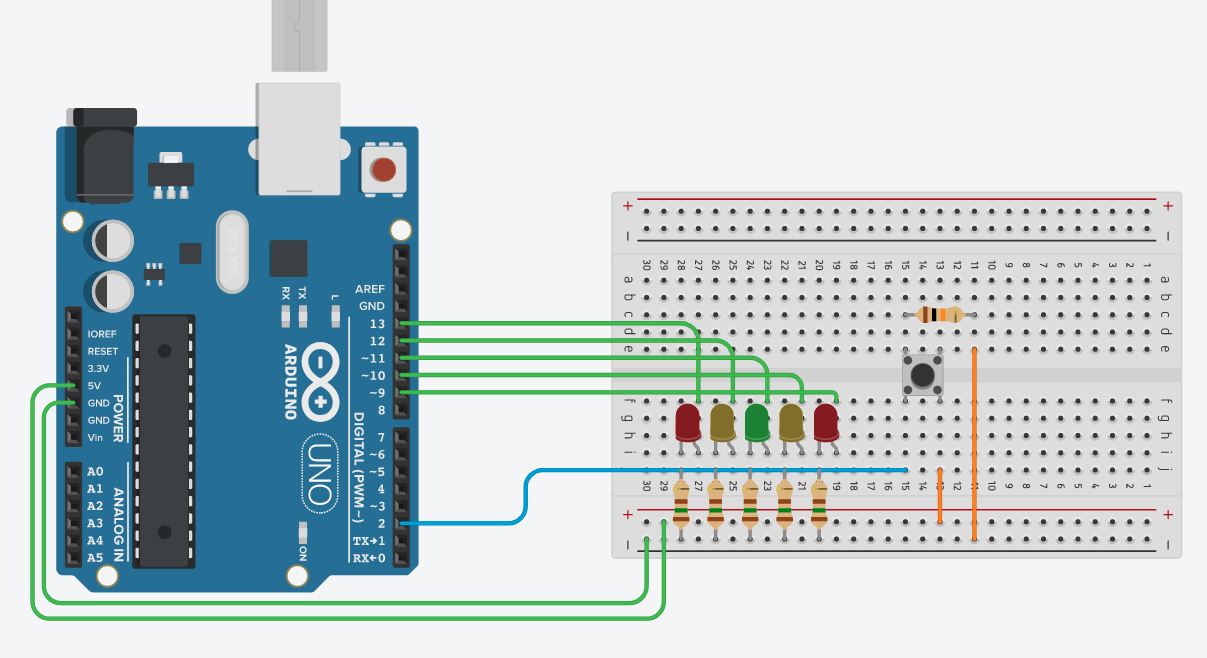
\includegraphics[width=\textwidth]{pictures/a2-praktik.png}
    \caption{Implementierter Stromkreis von Aufgabe 2}
    \label{fig:implementierter-stromkreis-a2}
\end{figure}

Weiters ist die Wahl der Pins zu erkennen.
Die Wahl viel auf die Pins 9 bis 13 zur Steuerung der LEDs und auf Pin 2 zur Erkennung des Tastendrucks.
Die Pins zur Ansteuerung der LEDs wurde willkürlich getroffen.
Es handelt sich nur von oben nach unten um die ersten, zur Verfügung stehenden Pins.
Pin 2 wurde gewählt, da nur Pin 2 und 3 in der Lage sind, an einen Interrupt gekoppelt zu werden.

Im Schaltkreis ist weiters der Taster zu sehen, der mit einem Pull-Up-Widerstand, wie in Sektion \ref{subsec:pullup} zu sehen, versehen ist.
Die Terminals an der Spalte 15 auf beiden Seiten sind verbunden, die Terminal an den Spalten 15 und 13 werden bei einem Tastendruck verbunden.
Damit ergibt sich das Teilschaltbild des Tasters, dass in Abbildung \ref{fig:schaltung-taster-pull-up} zu sehen ist.
Die alleinstehenden Zahlen geben die zugehörige Spalte des Steckbrettes an.
Des weiteren sei gesagt, dass in der Abbildung zwei Schalter zu sehen sind, diese repräsentieren die zwei vorhanden Terminals des echten Schalters.
Bei Tastendruck werden beide gleichzeitig geschlossen.

\begin{figure}[h]
    \centering
    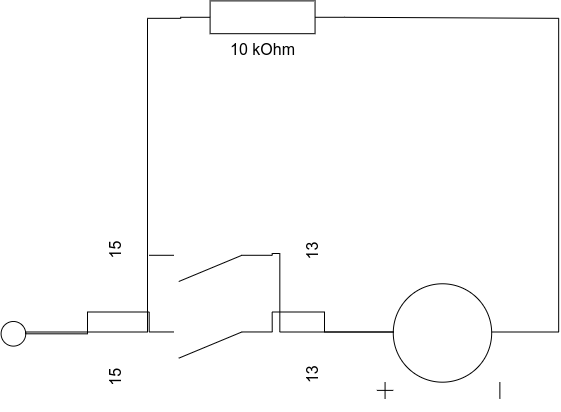
\includegraphics[width=0.58\textwidth]{pictures/a2-taster.png}
    \caption{Schaltung des Tasters mit Pull-Up Widerstand}
    \label{fig:schaltung-taster-pull-up}
\end{figure}

Im nachfolgendem Text wird der Programmcode der Aufgabe erläutert.
Einzelne Teile des Codes werden ausgewählt und beschrieben.
Am Ende dieser Sektion befindet sich der vollständige Programmcode.

\begin{lstlisting}[language=C,label={lst:a2-const-pin}, caption={Setzen der Pin-Konstanten}]
onst int NUM_PINS = 5;
const int WINNING_PIN_INDEX = 2;
const int PINS[] = {
	13, 12, 11, 10, 9
};
const int PIN_BUTTON = 2;
\end{lstlisting}

In Listing \ref{lst:a2-const-pin} werden die Nummern der Pins angelegt.
Die Besonderheit gegenüber der vorherigen Sektion, Sektion \ref{sec:aufgabe-1}, ist die Verwendung eines Arrays.
In diesem werden die verwendeten Pinnummern zu Ansteuerung der LEDs angegeben.
Mit $NUM\_PINS$ wird die Länge des Arrays angegeben.
Solch eine Angabe ist nützlich, da die Länge eines Arrays in der gegebenen Programmiersprache, C, nicht trivial findbar ist.

Um in C die Länge eines Arrays zu bestimmen, müsste zuerst mittels $sizeof(PINS)$ die Menge an Speicher ermittelt werden, die das Arrays belegt.
Dieser Wert müsste sodann durch das Ergebnis von $sizeof(int)$, die Menge an Speicher die ein Integer-Wert im Speicher belegt, dividiert werden.
Das Ergebnis aus $sizeof(PINS) / sizeof(int)$ würde dann die Länge des Arrays ergeben.
Einfacher ist es daher, die Größe als Konstante anzugeben, wenn diese, wie in diesem Fall, bekannt ist.
Mit der Konstante $PIN\:BUTTON$ wird die Pinnummer des Pins angegeben, welcher später den Zustand des Tasters erkennt.

\begin{lstlisting}[language=C,label={lst:a2-const-interval}, caption={Standard Interval zum LED wechsel}]
const unsigned long INTERVAL_DEFAULT = 5000;
\end{lstlisting}

Mit der Konstanten die in Listing \ref{lst:a2-const-pin} angegeben ist, wird das Standardinterval angegeben, mit dem bei den LEDs weitergesprungen wird.
D.h., nach Ablauf der Zeit von $INTERVAL\_DEFAULT$, in Millisekunden, wird zur nächsten LED gesprungen, wenn das Spiel neu gestartet wurde.


\begin{lstlisting}[language=C,label={lst:a2-zeitmessung-variablen}, caption={Variablen zur Zeitmessung}]
unsigned long current_millis = 0;
unsigned long previous_millis = 0;
unsigned long interval = INTERVAL_DEFAULT;
\end{lstlisting}

Die Variablen in Listing \ref{lst:a2-zeitmessung-variablen} werden dazu verwendet, die vergangene Zeit im Programm mitzuverfolgen.
In $current\_millis$ wird gespeichert, wie viel Zeit seit dem Programmstart vergangen ist.
Der Wert in $previous\_millis$ gibt an, zu welchem Zeitpunkt die letzte Aktion durchgeführt wird.
Die Bedeutung dieser Variable wird im Verlauf des Programmcodes klarer.
In $interval$ ist das derzeitige Interval zwischen Wechseln der LEDs gespeichert.
Zu Beginn wird sie mit der Konstante aus Listing \ref{lst:a2-const-interval} initialisiert.
Sie wird bei jedem Neustart des Spiels auf diesen Wert zurückgesetzt.

\begin{lstlisting}[language=C,label={lst:a2-game-state-variablen}, caption={Variablen zur Zustandsbestimmung des Spiels}]
int pin_index = 0;

volatile bool button_pressed = false;
volatile bool game_over = false;
\end{lstlisting}

Durch die Variablen in Listing \ref{lst:a2-game-state-variablen} wird der derzeitige Zustand des Spiels mitverfolgt.
Sie haben zusätzlich zum Typ noch das Schlüsselwort $volatile$, welches im zweiten Teil der Sektion \ref{subsec:a2-vorbereitunga} beschrieben wurde.
Diese Schlüsselwort benötigen sie, da die Variablen in einem Interrupt verändert werden und dadurch direkt vom Speicher ausgelesen werden müssen.
Eine Annäherung des mit diesen Variablen bewirkten Zustandsverlauf kann in Abbildung \ref{fig:annäherung-des-spielverlaufs} abgelesen werden.

\begin{figure}[ht]
    \centering
    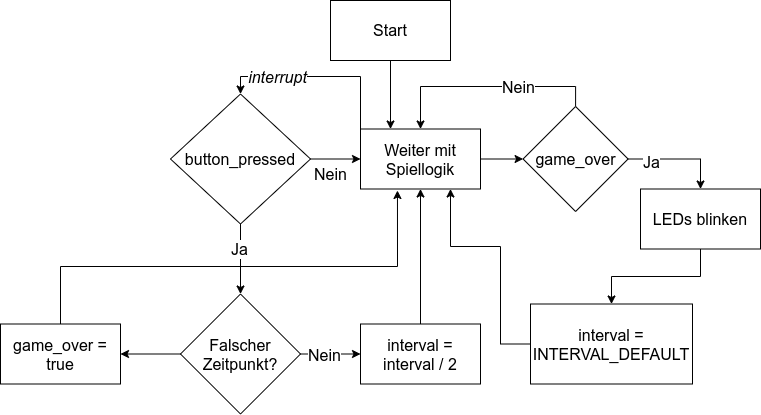
\includegraphics[width=\textwidth]{pictures/a2-game-state.png}
    \caption{Annäherung des Spielverlaufs}
    \label{fig:annäherung-des-spielverlaufs}
\end{figure}


Die Variable $pin\_index$ ist nicht mittels $volatile$ markiert, da sie sich nur in der Hauptschleife des Programms ändert.
Nach Ablauf von $interval$ wird sie um 1 erhöht bis zu einem Maximum von $NUM\_PINS - 1$.
Würde sie den Wert $NUM\_PINS$ annehmen, wird sie wieder auf 0 zurückgesetzt.
Diese Variable gibt an, welcher Index, von 0 beginnend, aus $PINS$ verwendet wird, um eine LED anzusteuern.
D.h., $pin\_index = 0 \Rightarrow \text Pin13 = HIGH$, $pin\_index = 1 \Rightarrow \text Pin12 = HIGH$, u.s.w..

\begin{lstlisting}[language=C,label={lst:a2-serial-begin}, caption={Einstellen der seriellen Schnittstelle}]
void setup() {
  Serial.begin(9600);
\end{lstlisting}




\begin{lstlisting}[language=C,label={lst:a1-loop}, caption={Vollständiger Programmcode für Aufgabe 2}]
const int NUM_PINS = 5;
const int WINNING_PIN_INDEX = 2;
const int PINS[] = {
	13, 12, 11, 10, 9
};
const int PIN_BUTTON = 2;
const unsigned long INTERVAL_DEFAULT = 5000;

unsigned long current_millis = 0;
unsigned long previous_millis = 0;
unsigned long interval = INTERVAL_DEFAULT;

int pin_index = 0;

volatile bool button_pressed = false;
volatile bool game_over = false;

void setup()
{
  Serial.begin(9600);

  int i;
  for (i = 0; i < NUM_PINS; i++) {
    pinMode(PINS[i], OUTPUT);
  }

  pinMode(PIN_BUTTON, INPUT_PULLUP);

  attachInterrupt(
    digitalPinToInterrupt(PIN_BUTTON),
    on_button_change,
    CHANGE);

  init_game();
}

void init_game() {
  game_over = false;
  interval = INTERVAL_DEFAULT;
  pin_index = 0;
  digitalWrite(PINS[0], HIGH);
}

void loop()
{
  current_millis = millis();

  if (current_millis - previous_millis >= interval
       && !button_pressed
       && !game_over) {
    digitalWrite(PINS[pin_index], LOW);
    increase_pin_index();
    digitalWrite(PINS[pin_index], HIGH);
	previous_millis = current_millis;
  } else if (game_over) {
    blink_all();
    init_game();
    previous_millis = current_millis;
  }
}

void blink_all() {
  int j;
  for (j = 0; j < 3; j++) {
    int i;
    write_to_all(HIGH);
    delay(500);
    write_to_all(LOW);
    delay(500);
  }
}

void write_to_all(int state) {
  int i;
  for (i = 0; i < NUM_PINS; i++) {
    digitalWrite(PINS[i], state);
  }
}

void increase_pin_index() {
    pin_index++;
    if (pin_index >= NUM_PINS){
      pin_index = 0;
    }
}

void on_button_change() {
  int button_state = digitalRead(PIN_BUTTON);
  if (button_state == HIGH) {
   	on_button_rising();
  } else {
    on_button_falling();
  }
}

void on_button_rising() {
  button_pressed = true;

  if (pin_index == WINNING_PIN_INDEX &&
     !game_over) {
    interval = interval / 2;
  } else {
    game_over = true;
  }
}

void on_button_falling() {
  button_pressed = false;
}
\end{lstlisting}


    \section{Aufgabe 3 - Realisierung eines Logic Analyzers}
\label{sec:aufgabe-3---realisierung-eines-logic-analyzers}

Es ist eine Schaltung zu entwerfen, welche Logikbausteine erkennt.
Da bei zwei Signalen $a$ und $b$ als Eingänge je nach Baustein, bzw.\ Gatter, ein anderes Signal $y$ am Ausgang anliegt, kann ein unbekanntes Gatter analysiert und benannt werden.


\subsection{Materialien}
\label{subsec:a3-materialien}

\begin{table}[h]
    \centering
    \caption{Aufgabe 3 - Verwendete Materialien}
    \label{tab:a3-materialien}
    \begin{tabular}{| l | l | l |}
        \hline
        Bezeichnung & Eigenschaften & Menge \\
        \hline
        Widerstand  & $150\Omega$   & 2     \\
        & Braun - Grün - Braun - Gold & \\
        74HC00 & NAND & 1 \\
        74HC02 & NOR  & 1\\
        74HC08 & AND & 1\\
        74HC32 & OR & 1\\
        74HC86 & XOR  & 1\\
        Mikrocontroller & Arduino Uno R3 & 1 \\
        \hline
    \end{tabular}
\end{table}


\subsection{Vorbereitung}
\label{subsec:a3-vorbereitung}

Zur Vorbereitung dieser Aufgabe, müssen die Wahrheitstabellen der zu untersuchenden Funktionen bekannt sein.
Dafür werden die Tabellen für die verwendeten Funktionen aufgestellt.
Es gilt die Annahme, dass die Funktionen bekannt sind und werden daher nicht näher erklärt.
Eine Erklärung der logischen Funktionen würde über den Umfang dieses Protokolls hinaus gehen.
Die Tabellen können in den Tabellen \ref{tab:wahrheitstabellen-verwendeter-logikfunktionen} angelesen werden.

\begin{table}[ht]
    \centering
    \caption{Wahrheitstabellen verwendeter Logikfunktionen}
    \label{tab:wahrheitstabellen-verwendeter-logikfunktionen}
    \begin{tabular}{| l | l || l |}
        \hline
        & AND & \\
        \hline
        A & B & Y \\
        \hline
        0 & 0 & 0 \\
        0 & 1 & 0 \\
        1 & 0 & 0 \\
        1 & 1 & 1 \\
        \hline
    \end{tabular}
    \quad
    \begin{tabular}{| l | l || l |}
        \hline
        & OR & \\
        \hline
        A & B & Y \\
        \hline
        0 & 0 & 0 \\
        0 & 1 & 1 \\
        1 & 0 & 1 \\
        1 & 1 & 1 \\
        \hline
    \end{tabular}
    \quad
    \begin{tabular}{| l | l || l |}
        \hline
        & NAND & \\
        \hline
        A & B & Y \\
        \hline
        0 & 0 & 1 \\
        0 & 1 & 1 \\
        1 & 0 & 1 \\
        1 & 1 & 0 \\
        \hline
    \end{tabular}
    \quad
    \begin{tabular}{| l | l || l |}
        \hline
        & NOR & \\
        \hline
        A & B & Y \\
        \hline
        0 & 0 & 1 \\
        0 & 1 & 0 \\
        1 & 0 & 0 \\
        1 & 1 & 0 \\
        \hline
    \end{tabular}
    \quad
    \begin{tabular}{| l | l || l |}
        \hline
        & XOR & \\
        \hline
        A & B & Y \\
        \hline
        0 & 0 & 0 \\
        0 & 1 & 1 \\
        1 & 0 & 1 \\
        1 & 1 & 0 \\
        \hline
    \end{tabular}
\end{table}

\subsection{Praktikumsaufgabe}
\label{subsec:a3-praktikumsaufgabe2}

Für die Aufgabe wurde nun die in Abbildung \ref{fig:a3-implementiert} gezeigte Schaltung implementiert.
Die Pins 13 und 12 bilden hierfür jeweils die Eingänge für das Logikgatter.
Der Pin 8 liest dann den Ausgang aus.
Die Widerstände von $150\Omega$ wurden verwendet, um die Logikbausteine vor zu hohen Stromflüssen zu schützen.
Mittels des angeschlossenen Multimeters kann der Ausgang manuell ausgelesen werden und das Ergebnis des Programmcodes überprüft werden.

\begin{figure}[ht]
    \centering
    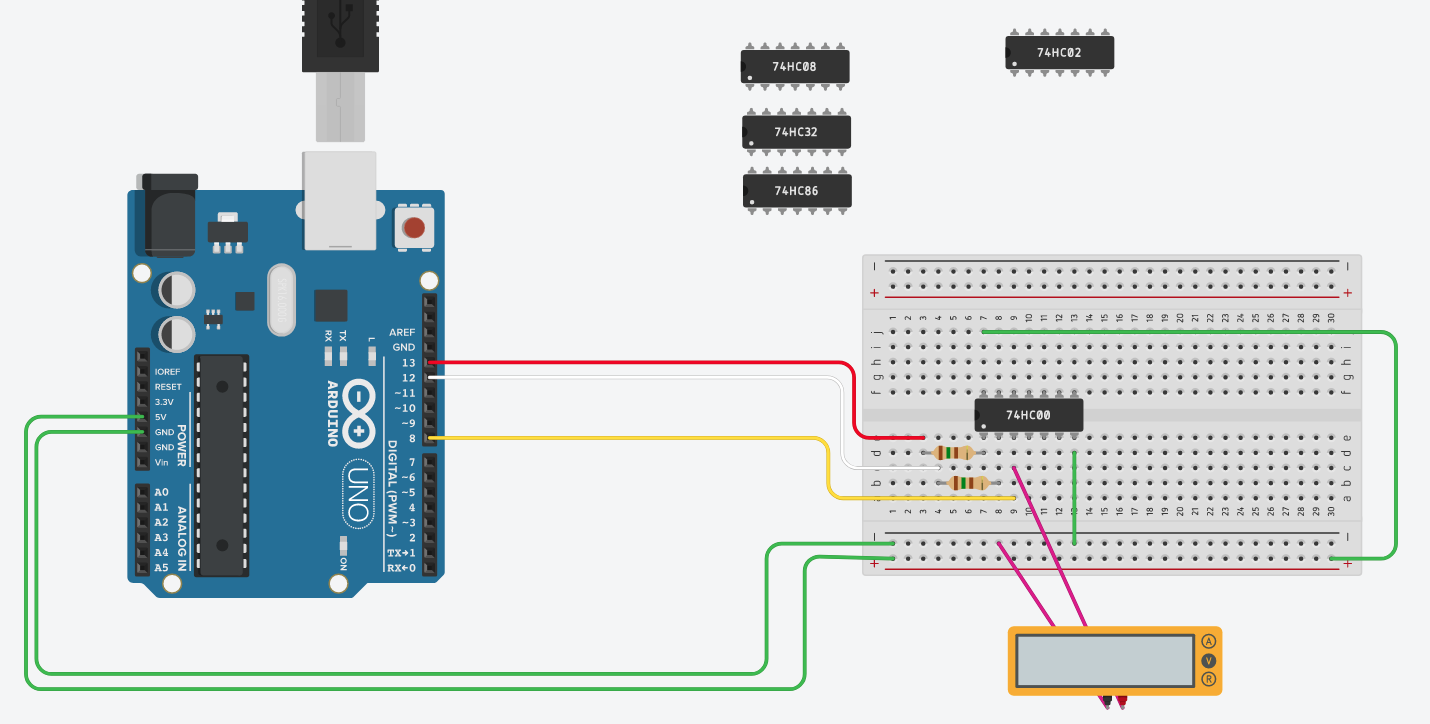
\includegraphics[width=\textwidth]{pictures/a3-praktik.png}
    \caption{Implementierter Stromkreis von Aufgabe 3}
    \label{fig:a3-implementiert}
\end{figure}

Im nachfolgendem Text wird der Programmcode der Aufgabe erläutert.
Einzelne Teile des Codes werden ausgewählt und beschrieben.
Am Ende dieser Sektion befindet sich der vollständige Programmcode.

\begin{lstlisting}[language=C,label={lst:a3-truthtable}, caption={Variable für die Wahrheitstabelle}]
/*
(Input1, Input2) => [Index]
(0, 0) => [0]
(0, 1) => [1]
(1, 0) => [2]
(1, 1) => [3]
*/
bool TRUTH_TABLE[] = { false, false, false, false };
\end{lstlisting}

In Listing \ref{lst:a3-truthtable} wird ein Array angelegt, welches die Ergebnisse der Evaluierung speichert.
Im Kommentar sind die Abbildungen der Eingänge auf den jeweiligen Index zu sehen.
D.h., werden beide Eingänge auf 0, bzw.\ $LOW$, geschalten, so wird das Ergebnis an Index 0 gespeichert.

\begin{lstlisting}[language=C,label={lst:a3-ausführen-des-gatters}, caption={Ausführen der Logikfunktionen}]
digitalWrite(PIN_OUTPUT_1, LOW);
digitalWrite(PIN_OUTPUT_2, LOW);

delay(2000);
TRUTH_TABLE[0] = digitalRead(PIN_INPUT) == HIGH;

digitalWrite(PIN_OUTPUT_1, LOW);
digitalWrite(PIN_OUTPUT_2, HIGH);

delay(2000);
TRUTH_TABLE[1] = digitalRead(PIN_INPUT) == HIGH;

digitalWrite(PIN_OUTPUT_1, HIGH);
digitalWrite(PIN_OUTPUT_2, LOW);

delay(2000);
TRUTH_TABLE[2] = digitalRead(PIN_INPUT) == HIGH;

digitalWrite(PIN_OUTPUT_1, HIGH);
digitalWrite(PIN_OUTPUT_2, HIGH);

delay(2000);
TRUTH_TABLE[3] = digitalRead(PIN_INPUT) == HIGH;
\end{lstlisting}

Der Code in Listing \ref{lst:a3-ausführen-des-gatters} setzt nacheinander die Eingänge des Gatters auf die Werte der Wahrheitstabellen.
D.h., es werden beide Eingänge auf 0 gesetzt und das Ergebnis im Array gespeichert.
Danach wird ein Eingang auf 1 und der andere auf 0 gesetzt und das Ergebnis wieder im Array gespeichert, u.s.w..

Zwischen den einzelnen Schaltungen der Eingänge wird mittels Aufruf von $delay(2000)$ zwei Sekunden lang gewartet.
Dieser Aufruf ist dazu da, um ein manuelles Ablesen des Multimeters zu ermöglichen und ist für die korrekte Ausführung des Programms nicht notwendig.

\begin{lstlisting}[language=C,label={lst:a3-aausgabe-der-wahrheitstabelle}, caption={Ausgabe der Wahrheitstabelle}]
Serial.println("");
Serial.println("|---|---|---|");
Serial.println("| a | b | y |");
Serial.println("|---|---|---|");

Serial.print("| 0 | 0 | ");
Serial.print(TRUTH_TABLE[0]);
Serial.println(" |");

Serial.print("| 0 | 1 | ");
Serial.print(TRUTH_TABLE[1]);
Serial.println(" |");

Serial.print("| 1 | 0 | ");
Serial.print(TRUTH_TABLE[2]);
Serial.println(" |");

Serial.print("| 1 | 1 | ");
Serial.print(TRUTH_TABLE[3]);
Serial.println(" |");
Serial.println("|---|---|---|");
Serial.println("");
\end{lstlisting}

Die Ergebnisse die in der Variable aus Listing \ref{lst:a3-truthtable} gespeichert wurden, werden in Listing \ref{lst:a3-aausgabe-der-wahrheitstabelle} ausgegeben.
Diese Ausgabe wird gemacht, um eine manuelle Überprüfung des Ergebnisses machen zu können.
D.h., sie wird gemacht um ein Debuggen des Codes zu ermöglichen, ist aber für eine korrekte Ausführung des Programms nicht notwendig.
Das Programm gibt hier die resultierende Wahrheitstabelle, in der Form einer Tabelle wie in Tabellen \ref{tab:wahrheitstabellen-verwendeter-logikfunktionen} dargestellt, aus.

\begin{lstlisting}[language=C,label={lst:a3-evaluierung-der-ergebnisse}, caption={Evaluierung der Ergebnisse}]
if (!TRUTH_TABLE[0]
&& !TRUTH_TABLE[1]
&& !TRUTH_TABLE[2]
&& TRUTH_TABLE[3]) {
    Serial.println("AND - Gate");
} else if (!TRUTH_TABLE[0]
&& TRUTH_TABLE[1]
&& TRUTH_TABLE[2]
&& TRUTH_TABLE[3]) {
    Serial.println("OR - Gate");
} else if (TRUTH_TABLE[0]
&& TRUTH_TABLE[1]
&& TRUTH_TABLE[2]
&& !TRUTH_TABLE[3]) {
    Serial.println("NAND - Gate");
} else if (TRUTH_TABLE[0]
&& !TRUTH_TABLE[1]
&& !TRUTH_TABLE[2]
&& !TRUTH_TABLE[3]) {
    Serial.println("NOR - Gate");
} else if (!TRUTH_TABLE[0]
&& TRUTH_TABLE[1]
&& TRUTH_TABLE[2]
&& !TRUTH_TABLE[3]) {
    Serial.println("XOR - Gate");
} else {
    Serial.println("Unrecognized Gate");
}
\end{lstlisting}

Die Ergebnisse werden in Listing \ref{lst:a3-evaluierung-der-ergebnisse} evaluiert.
Je nachdem welche Ausgaben der Logikbaustein getätigt hat, kann nun die entsprechende Funktion gefunden werden.
Dadurch wird das Ergebnis mit den Ergebnissen aus den Tabellen \ref{tab:wahrheitstabellen-verwendeter-logikfunktionen} verglichen.
Gleichen die Ergebnisse denen der Y-Spalte einer Tabelle, so wurde das jeweilige Gatter erkannt und der Name wird ausgegeben.
Sind die Ergebnisse nicht zuzuordnen, so wird die Meldung "Unrecognized Gate", zu Deutsch "Unbekanntes Gatter", ausgegeben.

\begin{lstlisting}[language=C,label={lst:a3-loop}, caption={Programmschleife}]
void loop()
{
}
\end{lstlisting}

Die Programmschleife in Listing \ref{lst:a3-loop} ist leer, da der Code für jedes Logikgatter nur einmal ausgeführt werden muss.
Da für jedes Logikgatter die Schaltung umgebaut werden muss, sprich, es muss das Gatter ausgetauscht werden, ist das Ausführen  des Codes in einer Schleife nicht zielführend.

\begin{lstlisting}[language=C,label={lst:a3-code}, caption={Vollständiger Programmcode der Aufgabe 3}]
const int PIN_OUTPUT_1 = 13;
const int PIN_OUTPUT_2 = 12;
const int PIN_INPUT = 8;

/*
(Input1, Input2) => [Index]
(0, 0) => [0]
(0, 1) => [1]
(1, 0) => [2]
(1, 1) => [3]
*/
bool TRUTH_TABLE[] = { false, false, false, false };

void setup()
{
  Serial.begin(9600);

  pinMode(PIN_OUTPUT_1, OUTPUT);
  pinMode(PIN_OUTPUT_2, OUTPUT);
  pinMode(PIN_INPUT, INPUT);

  digitalWrite(PIN_OUTPUT_1, LOW);
  digitalWrite(PIN_OUTPUT_2, LOW);

  delay(2000);
  TRUTH_TABLE[0] = digitalRead(PIN_INPUT) == HIGH;

  digitalWrite(PIN_OUTPUT_1, LOW);
  digitalWrite(PIN_OUTPUT_2, HIGH);

  delay(2000);
  TRUTH_TABLE[1] = digitalRead(PIN_INPUT) == HIGH;

  digitalWrite(PIN_OUTPUT_1, HIGH);
  digitalWrite(PIN_OUTPUT_2, LOW);

  delay(2000);
  TRUTH_TABLE[2] = digitalRead(PIN_INPUT) == HIGH;

  digitalWrite(PIN_OUTPUT_1, HIGH);
  digitalWrite(PIN_OUTPUT_2, HIGH);

  delay(2000);
  TRUTH_TABLE[3] = digitalRead(PIN_INPUT) == HIGH;

  Serial.println("");
  Serial.println("|---|---|---|");
  Serial.println("| a | b | y |");
  Serial.println("|---|---|---|");

  Serial.print("| 0 | 0 | ");
  Serial.print(TRUTH_TABLE[0]);
  Serial.println(" |");

  Serial.print("| 0 | 1 | ");
  Serial.print(TRUTH_TABLE[1]);
  Serial.println(" |");

  Serial.print("| 1 | 0 | ");
  Serial.print(TRUTH_TABLE[2]);
  Serial.println(" |");

  Serial.print("| 1 | 1 | ");
  Serial.print(TRUTH_TABLE[3]);
  Serial.println(" |");
  Serial.println("|---|---|---|");
  Serial.println("");

  Serial.println("Result: ");

  if (!TRUTH_TABLE[0]
      	&& !TRUTH_TABLE[1]
      	&& !TRUTH_TABLE[2]
      	&& TRUTH_TABLE[3]) {
    Serial.println("AND - Gate");
  } else if (!TRUTH_TABLE[0]
      	&& TRUTH_TABLE[1]
      	&& TRUTH_TABLE[2]
      	&& TRUTH_TABLE[3]) {
    Serial.println("OR - Gate");
  } else if (TRUTH_TABLE[0]
      	&& TRUTH_TABLE[1]
      	&& TRUTH_TABLE[2]
      	&& !TRUTH_TABLE[3]) {
    Serial.println("NAND - Gate");
  } else if (TRUTH_TABLE[0]
      	&& !TRUTH_TABLE[1]
      	&& !TRUTH_TABLE[2]
      	&& !TRUTH_TABLE[3]) {
    Serial.println("NOR - Gate");
  } else if (!TRUTH_TABLE[0]
      	&& TRUTH_TABLE[1]
      	&& TRUTH_TABLE[2]
      	&& !TRUTH_TABLE[3]) {
    Serial.println("XOR - Gate");
  } else {
    Serial.println("Unrecognized Gate");
  }
}

void loop()
{
}
\end{lstlisting}

\subsection{Fehlerdiskussion}
\label{subsec:a3-fehlerdiskussion}

Während des Testens des Programms konnten alle Gatter bis auf das NOR-Gatter nicht erkannt werden.
Der Grund dafür war, dass bei gleicher ausrichtung des NOR-Gatters, die Ein- und Ausgänge vertauscht waren.
D.h., die Reihenfolge der Pins der Bausteine war "Eingange 1 - Eingang 2 - Ausgang", außer am NOR-Gatter.
Hier ist die Reihenfolge "Ausgang - Eingang 1 - Eingang - 2".
Um das NOR-Gatter richtig zu erkennen, muss daher die Schaltung entsprechend angepasst werden.
Da die Schaltung theoretisch ein unbekanntes Gatter erkennen soll, müsste daher die Schaltung geändert werden, wenn das Gatter nicht erkannt wurde.
Wird das Gatter danach immer noch nicht erkannt, handelt es sich tatsächlich um ein unbekanntes Gatter, ansonsten um ein NOR-Gatter.

\subsection{Zusammenfassung}
\label{subsec:a3-zusammenfassung2}



    \section{Aufgabe 4 - Wertbestimmung von Widerstand und Kondensator}
\label{sec:aufgabe-4---wertbestimmung-von-widerstand-und-kondensator}

In dieser Aufgabe geht es um Widerstände und Kondensatoren.
Diese sind Grundbausteine der Elektrotechnik.
Neben diversen Berechnungen sind folgende Fragen zu beantworten.

\begin{itemize}
    \item Können Unterschiede zwischen Messungen am Mikrocontroller und manuellen Methoden gefunden werden?
    \item Wenn Ja, welche und warum?
    \item Mit welchen Prinzipien und Überlegungen wurden die Widerstände gemessen?
    \item Welche Abweichungen ergeben sich beim Messen bekannter Kondensatoren?
\end{itemize}

\subsection{Materialien}
\label{subsec:a4-materialien}

\begin{table}[h]
    \centering
    \caption{Aufgabe 4 - Verwendete Materialien}
    \label{tab:a4-materialien}
    \begin{tabular}{| l | l | l |}
        \hline
        Bezeichnung & Eigenschaften & Menge \\
        \hline
        Widerstand  & $10k\Omega$   & 2     \\
        & Braun - Schwarz - Orange - Gold & \\
        Widerstand & unbekannt & k.A. \\
        Kondensator & unbekannt & k.A \\
        Mikrocontroller & Arduino Uno R3 & 1 \\
        \hline
    \end{tabular}
\end{table}

In der Tabelle \ref{tab:a4-materialien} sind unbekannte Widerstände in nicht angegebener Menge gelistet.
Damit sind Testwiderstände gemeint, welche durch das Testen an der Schaltung gemessen werden können.
Beim Versuch an dieser Schaltung sind die Widerstandswerte normalerweise bekannt, um die Richtigkeit der Schaltung zu bestätigen.
Die Werte und Anzahl der verwendeten Widerstände sind jedoch nicht relevant.
Selbiges gilt für die Kondensatoren.

\subsection{Vorbereitung}
\label{subsec:a4-vorbereitung}

\subsubsection{Aufgabe 1}

In dieser Aufgabe sind Widerstände an Hand ihrer Farbcodes zu bestimmen.
Drei Widerstände sind gegeben.
Anhand der Tabelle in Sektion \ref{tab:farbcodierung-von-widerständen} kann der Wert bestimmt werden.

\begin{table}[ht]
    \centering
    \caption{Widerstandswerte}
    \label{tab:a4-widerstandswerte}
    \begin{tabular}{| l | l | l | l | l | l |}
        \hline
        Ring 1 & Ring 2 & Ring 3 & Ring 4 & Widerstandswert & Toleranz \\
        \hline
        Gelb & Violett & Rot & Gold & $4,7k\Omega$ & $\pm5\%$ \\
        Rot & Weiß & Grün & Gold & $3,9M\Omega$ & $\pm5\%$ \\
        Blau & Grau & Rot & Silber & $6,8k\Omega$ & $\pm10\%$ \\
        \hline
    \end{tabular}
\end{table}

\subsubsection{Aufgabe 2}

In Aufgabe 2 ist die Schaltung aus Abbildung \ref{fig:schaltung-a4-2} gegeben.

\begin{figure}[ht]
    \centering
    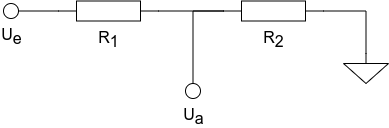
\includegraphics[width=\textwidth]{pictures/a4-1.png}
    \caption{Schaltung aus der Angabe aus Aufgabe 4.2}
    \label{fig:schaltung-a4-2}
\end{figure}

Für den ersten Teil sind folgende Werte gegeben.
\begin{itemize}
    \item $U_e = 5V$
    \item $U_a = 3V$
\end{itemize}

\newpage

Nun soll ermittelt werden, welches Verhältnis zwischen den Widerständen $R_1$ und $R_2$ herrschen muss, damit der gegeben Zustand möglich ist.
Um den Spannungsabfall über einen Widerstand zu ermitteln, kann die Formel des Spannungsteilers verwendet werden.

\begin{align}
    U_R = \frac{U}{R_{ges}} * R
\end{align}

Unter berücksichtigung der Angaben können die Werte eingesetzt werden.

\begin{align}
    U_a = \frac{U_e}{R_1 + R_2} * R_2
\end{align}

Nun kann umgeformt werden, um ein Verhältnis zwischen $R_2$ und $R_{ges}$ zu erhalten.

\begin{align}
    U_a = \frac{U_e}{R_1 + R_2} * R_2 \Rightarrow\\
    \frac{U_a}{U_e} = \frac{R_2}{R_{ges}} \Rightarrow\\
    \frac{3}{5} = \frac{R_2}{R_{ges}}
\end{align}

Daher gilt:

\begin{align}
    \frac{3}{5} = \frac{R_2}{R_{ges}} \Rightarrow \frac{2}{5} = \frac{R_1}{R_{ges}} \Rightarrow \\
    \frac{3}{5} * R_{ges} = R_2 \text{ und } \frac{2}{5} * R_{ges} = R_1 \Rightarrow
\end{align}

Das Verhältnis zwischen den Widerständen kann nun berechnet werden.

\begin{align}
    \frac{R_1}{R_2} = \\
    \frac{\frac{2}{5} * \cancel{R_{ges}}}{\frac{3}{5} * \cancel{R_{ges}}} = \\
    \frac{\frac{2}{\cancel{5}}}{\frac{3}{\cancel{5}}} = \\
    \frac{2}{3}
\end{align}

Nun muss berechnet werden, wie hoch der Widerstand $R_2$ sein muss, wenn $R_1 = 10k\Omega$ gilt.

\begin{align}
    (10) \land (13) \Rightarrow \\
    \frac{R_1}{R_2} = \frac{2}{3} \Rightarrow \\
    \frac{3 * 10k\Omega}{2} = R_2 = 15k\Omega
\end{align}

Nun soll ein unbekannter Widerstand $R_x$ berechnet werden, wenn $R_1 = 10k\Omega$ und $U_a = 1V$ gilt.
Für den Spannungsteiler gilt nun folgendes.

\begin{align}
    U_a = \frac{U_e}{R_x + R_1} * R_x \Rightarrow \\
    U_e = \frac{U_a * (R_x + R_1)}{R_x} \Rightarrow \\
    \frac{U_e}{U_a} = \frac{R_x}{R_x} + \frac{R_1}{R_x} \Rightarrow \\
    \frac{U_e}{U_a} - 1 = \frac{R_1}{R_x} \Rightarrow \\
    R_x = \frac{R_1}{\frac{U_e}{U_a} - 1} \Rightarrow \\
    R_x = \frac{R_1}{\frac{U_e - U_a}{U_a}} \Rightarrow\\
    R_x = \frac{\frac{R_1 * U_a}{U_a}}{\frac{U_e - U_a}{U_a}} \Rightarrow \\
    R_x = \frac{R_1 * U_a}{U_e - U_a}
\end{align}

Durch einsetzen der gegebenen Werte ergibt sich nun ein Wert für $R_x$.

\begin{align}
    (24) => \\
    R_x = \frac{R_1 * U_a}{U_e - U_a} = \\
    \frac{10k\Omega * 1V}{5V - 1V} = \\
    \frac{10k\Omega V}{4V} \Rightarrow \\
    R_x = 2,5k\Omega
\end{align}

\newpage

\subsubsection{Aufgabe 3}

In dieser Aufgabe wird ein Kondensator über einen Wiederstand $R = 10k\Omega$ an einer Spannungsquelle $U_q$ geladen.
Die Spannung des Kondensators ist $U_c(0) = 0V$ und $U_c(0,1s) = 0,63 * U_q$.
Es soll die Kapazität des Kondensators ermittelt werden.

Die Formel zur Berechnung der Spannung des Kondensators lautet folgendermaßen.

\begin{align}
    U_c(t) = \frac{1}{C} * I * t
\end{align}

Dies kann folgendermaßen umgeformt werden.

\begin{align}
    U_c(t) = \frac{1}{C} * I * t = \\
    \frac{1}{C} * \frac{U_q}{R} * t \Rightarrow \\
    C = \frac{U_c(t)}{\frac{U_q}{R} * t}
\end{align}

Nun können die Werte der Angabe eingesetzt werden.

\begin{align}
    (33) \Rightarrow \\
    C = \frac{0,63 * U_q}{\frac{U_q}{10k\Omega} * 0,1s} = \\
    \frac{0,63}{\frac{1}{10k\Omega} * 0,1s} = \\
    15\mu F
\end{align}

Nun soll ermittelt werden, wie lange es dauert, denn Kondensator vollständig zu laden.
Wir wissen:

\begin{align}
    \tau = RC \Rightarrow \\
    \tau = 0,15s
\end{align}

Weiters ist bekannt

\begin{align}
    U_c \geq 0,99U_Q \Leftrightarrow \text{nach } 5\tau
\end{align}

daraus folgt

\begin{align}
    t_{99\%} = 5\tau = 0,75s
\end{align}

\subsection{Praktikumsaufgabe}
\label{subsec:a4-praktikumsaufgabe2}

\subsubsection{Aufgabe 1}

Es wurde die in Abbildung \ref{fig:a4-1-implemtierung} gezeigte Schaltung implementiert.
Am Steckbrett ist eine ähnliche Schaltung wie in Abbildung \ref{fig:schaltung-a4-2} zu sehen.
Der Pin A0 ist zwischen den bekannten $10k\Omega$ und den unbekannten Widerstand geschaltet.
Nun sind folgende WGrößen bekannt.

\begin{itemize}
    \item $V_{out}$ des Mikrocontrollers $V_{out} = 5V$
    \item Der bekannte Widerstand zwischen $V_{out}$ und A0, $R_1 = 10k\Omega$
\end{itemize}

Durch die Überlegung von (26) kann im Mirocontroller ein Programm implementiert werden, welches den unbekannten Widerstand errechnet.

\begin{figure}[ht]
\centering
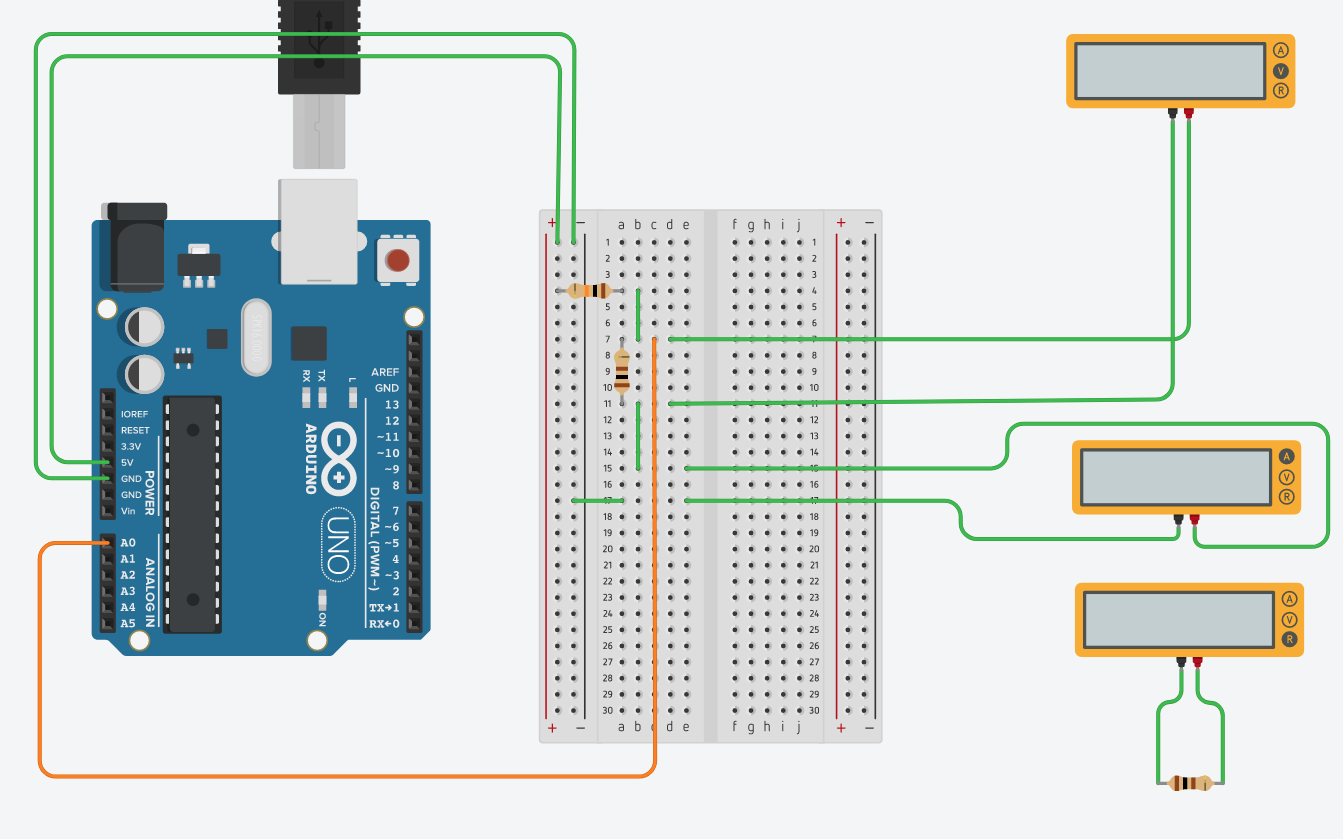
\includegraphics[width=\textwidth]{pictures/a4-1-praktik.png}
\caption{Implementierter Stromkreis von Aufgabe 4.1}
\label{fig:a4-1-implemtierung}
\end{figure}

Im nachfolgendem Text wird der Programmcode der Aufgabe erläutert.
Einzelne Teile des Codes werden ausgewählt und beschrieben.
Am Ende dieser Sektion befindet sich der vollständige Programmcode.

\begin{lstlisting}[language=C,label={lst:a4-1-konstanten}, caption={Konstanten der Aufgabe 4.1}]
const int PIN_VOLTAGE = A0;
const float U_IN = 5;
const float RESOLUTION = U_IN / 1024;
const int RESISTOR = 10 * 1000;
\end{lstlisting}

Durch den Code in Listing \ref{lst:a4-1-konstanten} werden die bekannten Größen angelegt.
\textit{U\_IN} gibt die Spannung in Volt an, während \textit{RESISTOR} den Widerstandswert abbildet.
Die Konstante \textit{RESOLUTION} bedarf genauerer Erklärung.

Die analogen Pins des Microkontroller können Spannungen zwischen 0V und 5V auslesen.
Um diese als Zahl darzustellen, wird ein Wert zwischen 0 und 1024 zurückgegeben.
Hierbei steht 0 für 0V und 1024 für 5V.
Das Interval $(0V, 5V)$ wird daher auf das Interval $(0, 1024)$ abgebildet.
Um die Spannung nun in Volt zu erhalten, muss mit der Wert aus A0 mit $\frac{5V}{1024}$ multipliziert werden.
Dieser Multiplikator wird in der Konstante \textit{RESOLUTION} gespeichert.

Der verwendete Microkontroller konfiguriert analoge Pins standardmäßig als Input-Pins.
Eine explizite Konfiguration als solche in der $setup()$ Funktion ist also nicht notwendig.

\newpage

\begin{lstlisting}[language=C,label={lst:a4-1-loop}, caption={Programmschleife der Aufgabe 4.1}]
void loop()
{
    int value = analogRead(PIN_VOLTAGE);
    float u_a = value * RESOLUTION;
    float r = (u_a * RESISTOR) / (U_IN - u_a);

    Serial.println("");
    Serial.print(u_a);
    Serial.println(" V");
    Serial.print(r);
    Serial.println(" Ohm");
    delay(1000);
}
\end{lstlisting}

In Listing \ref{lst:a4-1-loop} wird zuerst der derzeitige Wert des Pins A0 ausgelesen und in der variable \textit{value} abgelegt.
Dieser Wert wird nun mit den in Listing \ref{lst:a4-1-konstanten} angelegten Multiplikator \textit{RESOLUTION} multipliziert, um die Spannung $U_a$, vergleiche \ref{fig:stromkreis-a1}, zu erhalten.
Durch die Überlegung aus (mal26) kann nun der Widerstand $R_2$, bzw. $R_x$, errechnet werden.

Danach erfolgt die Ausgabe über der errechneten Größen über die serielle Schnittstelle.
Ein Pausieren des Programms wird durchgeführt, um ein angenehmeres Lesen der Ausgabe zu ermöglichen.

\newpage

\begin{lstlisting}[language=C,label={lst:a4-1-programmcode}, caption={Vollständiger Programmcode der Aufgabe 4.1}]
const int PIN_VOLTAGE = A0;
const float U_IN = 5;
const float RESOLUTION = U_IN / 1024;
const int RESISTOR = 10 * 1000;

void setup()
{
    Serial.begin(9600);
}

void loop()
{
    int value = analogRead(PIN_VOLTAGE);
    float u_a = value * RESOLUTION;
    float r = (u_a * RESISTOR) / (U_IN - u_a);

    Serial.println("");
    Serial.print(u_a);
    Serial.println(" V");
    Serial.print(r);
    Serial.println(" Ohm");
    delay(1000);
}
\end{lstlisting}

\subsubsection{Aufgabe 2}

In dieser Aufgabe, soll die Kapazität eines Kondensators ermittelt werden.
Es wurde die Schaltung aus Abbildung \ref{fig:implementierung-aufgabe-4-2} implementiert.
Im Unterschied zur Schaltung aus Abbildung \ref{fig:a4-1-implemtierung}, wurde der unbekannte Widerstand durch einen Kondensator ersetzt, welcher eine unbekannte Kapazität besitzt.

\begin{figure}[h]
    \centering
    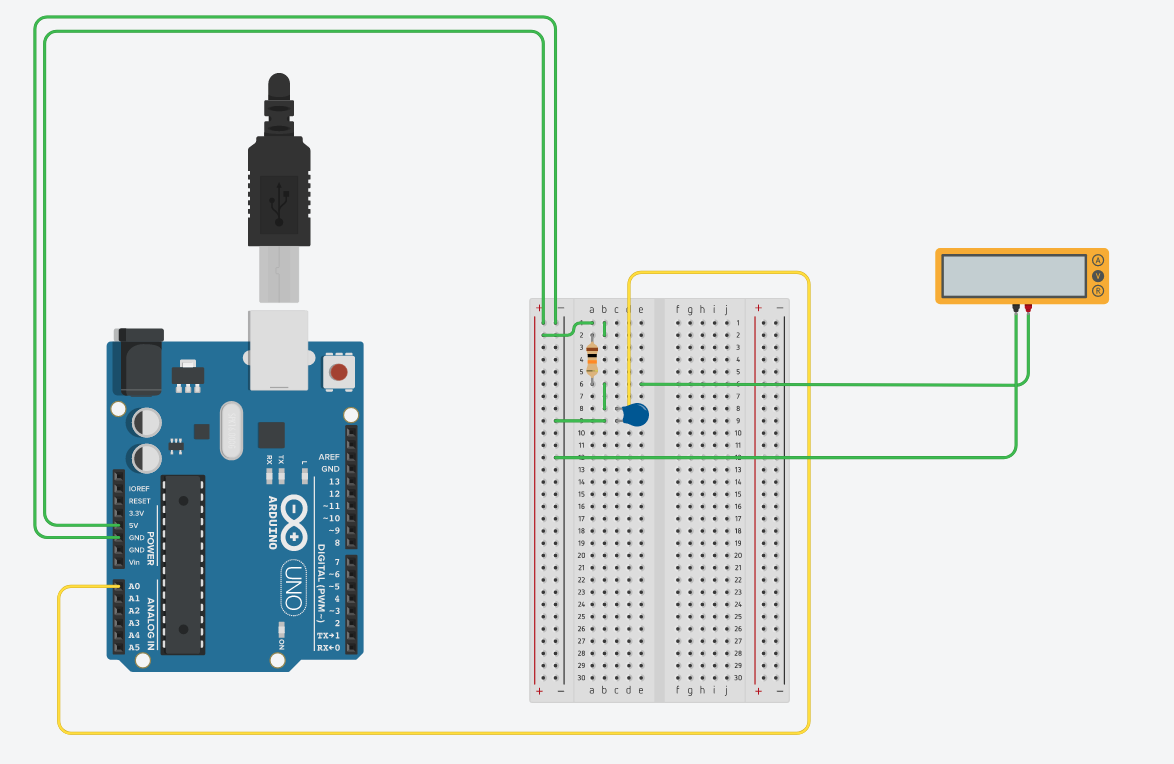
\includegraphics[width=0.9\textwidth]{pictures/a4-2-pratik.png}
    \caption{Implementierter Stromkreis von Aufgabe 4.2}
    \label{fig:implementierung-aufgabe-4-2}
\end{figure}

Im nachfolgendem Text wird der Programmcode der Aufgabe erläutert.
Einzelne Teile des Codes werden ausgewählt und beschrieben.
Am Ende dieser Sektion befindet sich der vollständige Programmcode.

\begin{lstlisting}[language=C,label={lst:a4-2-preprozessor-anweisung}, caption={Preprozessoranweisung}]
#include <math.h>
\end{lstlisting}

\newpage

In Listing \ref{lst:a4-2-preprozessor-anweisung} wurde eine Preprozessoranweisung verwendet.
Diese fügt eine C-Bibliothek hinzu, die verschiedene mathematische Funktionen zur Verfügung stellt.
Die Funktion die in dieser Aufgabe verwendet wurde, ist die $log()$ Funktion.
Es werden außerdem die selben Konstanten wie in Listing \ref{lst:a4-1-konstanten} verwendet.

\begin{lstlisting}[language=C,label={lst:a4-2-programloop}, caption={Programmschleife}]
double c = 0.0;

void loop()
{
  int value = analogRead(PIN_VOLTAGE);
  double u_a = value * RESOLUTION;

  if (u_a < 3.6) {
    double t = (double)millis() / 1000.0;
    if (u_a > 0) {
    	c = -t / (log(1 - (u_a / U_IN)) * RESISTOR);
        Serial.print(c, 6);
        Serial.println(" F");
    }
  }
}
\end{lstlisting}

Im Listing \ref{lst:a4-2-programloop} wird nun die Kapazität berechnet.
Dafür wird zusätzlich zum Wert des Pins A0 die vergangene Zeit miteinbezogen.
Die Berechnung der Kapazität ergibt sich aus folgender Überlegung.

Die Formel der Spannung eines Kondensators ist gegeben durch:

\begin{align}
    U_c(t) = U * (1 - e^{\frac{-t}{RC}})
\end{align}

Durch Umformen kann auf die Kapazität C umgeformt werden.

\begin{align}
    U_c(t) = U * (1 - e^{\frac{-t}{RC}}) \Rightarrow \\
    \frac{U_c(t)}{U} - 1 = -e^{\frac{-t}{RC}} \Rightarrow \\
    ln(1 - \frac{U_c(t)}{U}) = \frac{-t}{RC} \Rightarrow \\
    \frac{log_{10}(1 - \frac{U_c(t)}{U}) R}{-t} = \frac{1}{C} \Rightarrow \\
    C = \frac{-t}{log_{10}(1 - \frac{ U_c(t)}{U}) R}
\end{align}

Um ein akkurates Ergebnis zu erhalten, wird die Formel under den folgenden Bedingungen verwendet.
Die Spannung am Kondensator $u\_a$ muss unter $3,6V$ betragen, aber höher als $0V$ sein.
Letztere Bedingung wurde gewählt, da ansonsten eine Division durch $0$ möglich wäre.
Erstere, da beim Testen des Programms festgestellt wurde, dass die errechnete Kapazität mit fortschreitender Zeit ungenauer, bzw.\ falsch wurde.
Der in Listing \ref{lst:a4-2-programloop} verwendete Wert von $3,6V$ wurde verwendet, da dieser in der Ausgabe am Monitor den genauesten Wert zu liefern schien.

\newpage

\begin{lstlisting}[language=C,label={lst:a4-2-programmcode}, caption={Vollständiger Programmcode der Aufgabe 4.2}]
#include <math.h>

const int PIN_VOLTAGE = A0;

const double U_IN = 5;
const double RESOLUTION = U_IN / 1024;
const double RESISTOR = 10 * 1000;

double c = 0.0;

void setup()
{
  Serial.begin(9600);
}

void loop()
{
  int value = analogRead(PIN_VOLTAGE);
  double u_a = value * RESOLUTION;

  if (u_a < 3.6) {
    double t = (double)millis() / 1000.0;
    if (u_a > 0) {
    	c = -t / (log(1 - (u_a / U_IN)) * RESISTOR);
        Serial.print(c, 6);
        Serial.println(" F");
    }
  }
}
\end{lstlisting}

\subsection{Fehlerdiskussion}
\label{subsec:a4-fehlerdiskussion}

Für die Berechnung der Kapazität wurde zuerst die Überlegung aus (33) verwendet.
Die Verwendung dieser Formel führte jedoch zu unbefriedigenden Messungen und wurde mit der Überlegung aus (47) ersetzt.
Diese führte ebenso zu unbefriedigenden, jedoch genaueren Werten als (33).
Erst als das Limit von $u\_a < 3,6$ eingeführt wurde, wurden befriedigende Messergebnisse erzielt.
Womöglich könnte mit dieser Einschränkung auch mit (33) ein gleich gutes Ergebnis erreicht werden.

\begin{figure}[ht]
    \centering
    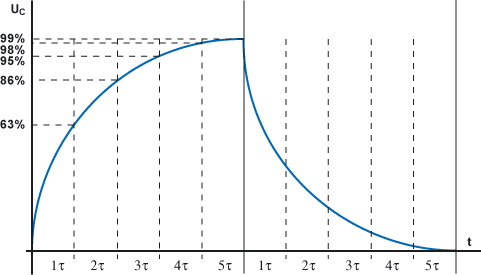
\includegraphics[width=\textwidth]{pictures/Kondensator-Ladekurve.png}
    \caption{Lade- und Entladekurve eines Kondensator \cite{kondesator}}
    \label{fig:lade-entladekurve-kondensator}
\end{figure}

\newpage

Des weiteren wurde der Wert von $3,6V$ für die Obergrenze von $u\_a$ durch experimentieren, d.h., willkürlich, festgelegt.
Nachdem der Wert von $3,6$ nahe an $0,63U = 0,63*5V = 3,15V$ liegt, ist es naheliegend das ein weniger willkürlicher Wert $3,15V$ sein könnte.
Dieser Wert ergibt sich aus der Spannung am Kondesator nach dem er $1\tau$ lang, siehe Abbildung \ref{fig:lade-entladekurve-kondensator}, geladen wurde.


    \addcontentsline{toc}{section}{References}
    \printbibliography
\end{document}
